%
% Theory
%

% !TEX root = ../../main.tex

\chapter{Grundlagen}

\section{Natural Evoltions vs Artifical}
  Natürliche Evolution hat kein vordefiniertes Ziel und ist ein sogennanter open-ended Anpassungsprozess. Artifizielle Evolution jedoch ist ein Optimierungsprozess, welcher versucht Lösungen zu vordefinierten Problem zu finden \cite[S.1]{book:bioInspired}. \\

\section{Genotype}
  (vieleicht nicht nötig so genau auf die biologischen zwecke einzugehen, hat bis jetzt nicht immer zu guten Ergebnissen geführt wenn man sich daran hält)
  The genetic material of an individual is known as the genotype, whereas its manifestation as an organism is known as the phenotype. Cells contain a class of molecules, known as proteins, whose shape,
  concentration, and behavior determine the properties of the cell. For example hair cells and muscle cells are different because they are composed of different proteins. \\
  The definition of specific proteins depends on another molecule, known as DNA (deoxyribonucleic acid), which in turn relies on proteins to become operative and on the mediation of a third type of molecule,
  known as RNA (ribonucleic acid), which is structurally similar to the DNA molecule. The DNA is the genetic material that is transmitted over generations.
  It is often enclosed within the nucleus of the cell and all cells in the organism have the same genetic material. \\
  DNA molecules are long chains of complementary strands composed of four types of chemical units(nucleotides or bases): adenine (A), cytosine (C), guanine (G), and thymine(T). \\
  The two strands stick together because nucleotides can lock to each other: Adenine binds to thymine and cytosine binds to guanine. This specific binding means that the two DNA strands are perfectly complementary. \\
  The genetic material is organized in several separated DNA molecules, called chromosomes. There are two types of cell replication: mitosis and meiosis. \\
  Mitosis occurs during growth of the organism when a cell divides by producinga copy with the same number of chromosomes (23 times 2 in humans).
  During mitosis, the two strands of the 46 DNA molecules are separated and each strand goes to one cell. Each strand then rebuilds the missing strand by recruiting the complementary nucleotides.
  The process ends with two exact copies of the double-stranded DNA molecule, one for each cell.
  Meiosis occurs during the production of sex cells (sperm and eggs). Sex cells receive only one chromosome for each pair. \\
  In diploid organisms the pairs of chromosomes are recombined during fecundation of the egg cell (containing the set of chromosomes from the mother) by the sperm cell (containing the set of chromosomes from the father).
  \cite[S.5 - 7]{book:bioInspired}.

\section{Gene Expression}
  (vieleicht nicht nötig so genau auf die biologischen zwecke einzugehen, hat bis jetzt nicht immer zu guten Ergebnissen geführt wenn man sich daran hält)
  The sequence of four nucleotides along the DNA chain determines the properties of the cells and the development of the organism. The four nucleotides are effectively the letters of the genetic alphabet.
  Genes are functionally relevant subsequences of nucleotides in the DNA chain (just like words in a sentence), which can produce proteins.
  Proteins are long molecular chains composed of hundreds of submolecules, known as amino acids.  The properties of a protein are determined mainly by its shape. Each amino acid corresponds to one or
  more specific sequences of three nucleotides (codon) in the DNA chain. The production of proteins \ref{pic:dnaTranscription} from DNA is mediated by RNA.
  RNA is a long molecule similar to DNA, but it consists of only one strand of nucleotides, is much shorter (typically a few thousand nucleotides), and features uracil (U) in place of DNA thymine (T).
  During protein production, the two strands of DNA are separated and an RNA molecule is assembled along a small part of the DNA strand so as to match the corresponding nucleotides.
  This process is known as transcription. The resulting RNA molecule is used to create a protein by assembling a chain of amino acids that correspond to the sequence of nucleotides.
  Some proteins regulate cell division and genetic expression of proteins. It is important to notice that while the sequence of DNA nucleotides cannot be modified by proteins, the sequence of protein amino
  acids is instead determined by DNA. In other words, information flows in one direction only, from genes to proteins. This is the reason why modifications of the phenotype that occur during the life of the individual and are
  caused by environmental phenomena cannot directly modify the genotype and be inherited by offspring (with the exception of exposure to radiation, which can directly affect the DNA sequence).
  \begin{figure}
    \centering
    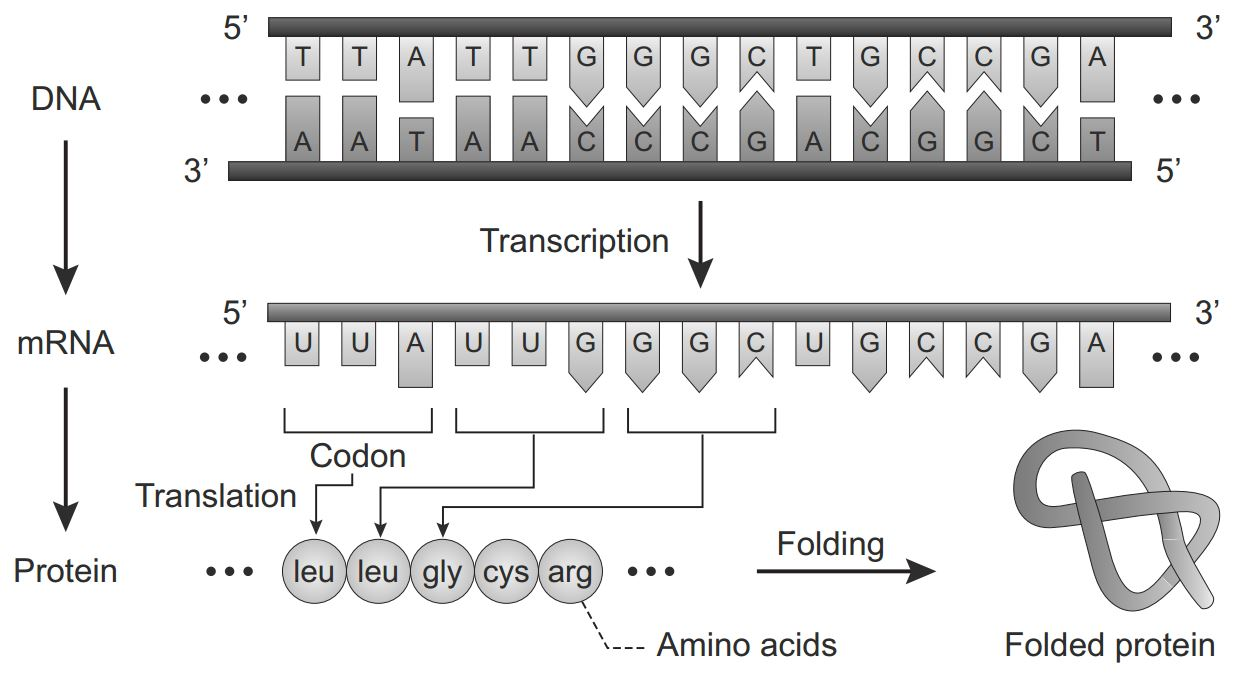
\includegraphics[width=10cm]{./graphics/DNA_Transcription_Protein}
    \caption[DNA Transcription]{DNA Transcription Prozess}
    \label{pic:dnaTranscription}
  \end{figure}

\section{Genetic Mutations}
  Muss mann sicher auch noch erwähnen.

\section{Artifical Evolution}

  \subsection{Evolutionärer Algorithmus erstellen}
  \label{sub:evAlgoErstellen}
    Nach \cite[S.16 - 29]{book:bioInspired}:
    \begin{itemize}

      \item Auswahl einer genetischen Repräsentation
        \begin{itemize}
          \item Diskrete Repräsentation [ABCDEF], [0111110]
          \item Reale Werte Pepräsentation 12.1245
          \item Baum Repräsentation \Tree [.A [.B [.C eins ] [.D zwei ] ].B [.E {3 und 4} ] ].A
        \end{itemize}

      \item Population erstellen
          \begin{itemize}
            \item Die Grösse der Population hängt von den Eigenschaften des Suchraums und der Rechenkosten der Evaluation ab
            \item Möglich viele unterschiedliche Individuen generieren
          \end{itemize}

      \item Fitnessfunktion definieren
        \begin{itemize}
          \item Auswahl und Kombination der Fitnesskomponenten
          \item Wie wird die Funktion evaluiert?
        \end{itemize}

      \item Auswahloperation definieren
        \begin{itemize}
          \item Ziel: Möglichst viele gute Individuen selektieren um Nachkommen der nächsten Generation zu erzeugen
          \item Selection Pressure
            \begin{itemize}
              \item Prozentsatz der Population die verwendet wird um Nachkommen zu reproduzieren, bsp 0.2
              \item Vorteil: Schnelle Verbesserung der Fitnessfunktion
              \item Nachteil: Schwierig Diversität zu erhalten
            \end{itemize}
          \item Proportinate Selection
            \begin{itemize}
              \item Reproduktionsrate proportinal zur Fitnessfunktion
              \item Nachteil: Schlecht wenn alle Indivduen gleiche Fitnesswerte vorweisen oder es nur einen Ausreisser gibt
            \end{itemize}
          \item Rank-based Selection
            \begin{itemize}
              \item Individuen Rangliste erstellen und Reproduktionswahrscheinlichkeiten proportional zu Rang zu ordnen
              \item Vorteil: Da die Reproduktionswahrscheinlichkeit proportinal zum Rang ist, kommt es nicht drauf an wie wenig unterschiedlich die Individuen sind.
            \end{itemize}
          \item Truncated Rank-based Selection: Nur die besten Individuen der Rangliste zur Reproduktion selektieren. Im Gegensatz zu Rank-based Selection erzeugt jedes Individuum die gleiche Anzahl Nachkommen.
          \item Tournament-basd Selection
            \begin{itemize}
              \item Wähle k zufällige Individuen, das Individuum mit der höchsten Fitness erzeugt Nachkommen
              \item Vorteil: Gute Balance zwischen Selection-Pressure und genetischer Diversität
            \end{itemize}
          \item Generational Replacement
            \begin{itemize}
              \item Die ganze Population wird durch Nachkommen ersetzt
              \item Elitism kann helfen den Prozess zu verbessern in dem immer die n besten Individuen erhalten bleiben
            \end{itemize}


        \end{itemize}

      \item Rekombinationsfunktion definieren
        \begin{itemize}
          \item Paarweise seletkion der Nachkommen
          \item Gene der Paare werden rekombiniert (untereinander vertauscht)
          \item One-Point Crossover
            \begin{itemize}
              \item Zufällige Bestimmung eines Cross-Over Punktes an dem die Gene des Paares vertauscht werden.
              \item Anwendbar auf Diskrete und Reale Werte Repräsentationen
            \end{itemize}
          \item Multi-Point Crossover: Gleich wie One-Points, es werden aber mehrere Cross-Over Punkte bestimmt
          \item Uniform Crossover
            \begin{itemize}
              \item Vertauschen von Genen an n zufälligen Positionen
              \item Anwendbar auf Reale Werte Repräsentationen
            \end{itemize}
          \item Arithemtic Crossover
            \begin{itemize}
              \item Durchschnitte von Genen an n zufälligen Positionen
              \item Es wird nur ein Nachkomme generiert
              \item Anwendbar auf Reale Werte Repräsentationen
            \end{itemize}
          \item Sequenzen : Es wird ein neuer Nachkomme gebildet unter Einhalten von Regeln. Alle Einträge dürfen nur Einmal vorkommen etc.... Unique Version von Multi-Point Crossover.
          \item Rekombinations bei Baum Repräsentationen: Es werden nur zufällige Teile des Baumes unter den Paaren vertauscht.
        \end{itemize}

      \item Mutationsfunktion definieren
        \begin{itemize}
          \item Mutationen operieren auf Level Indivduum
          \item Es ist Vorsicht geboten, da gefundene Lösungen durch Mutationen verloren gehen können
          \item Positionen eine Genomes werden mit einer bestimmten Wahrscheinlichkeit \(p_{m}\) mutiert.
          \item Binär: Flippen der Bits
          \item Reale Werte Repräsentation: Addieren eines zufälligen Wertes aus einer Gaus Verteilung \(N(0,\sigma)\)
          \item Sequenzen: Zufälliges austauschen Zweier Positionen
          \item Baum: Mutieren von Nodes. Gleiches Alphabet verwenden.
        \end{itemize}

      \item Ergebniss Analysemethode definieren
    \end{itemize}

    Genetische Representation: Erbgutdaten, genetic encoding \\
    Phenotyp: Aussehen des Individum -> Manifestation. In unserem Fall die 6-Beinigen Kreaturen als Pixelgrafik. \\
    Initialisieren -> Simulieren -> Selection -> Rekombination -> Mutation -> Analyse \\
    Simulieren bis Analayse solange wiederholen bis zufrieden mit Resultat


  \subsection{Arten von evolutionären Algorithmen}
  \label{sub:artenEvAlgos}
    \begin{itemize}
      \item Genetische Algorithmen
      \label{item:genAlgo}
        \begin{itemize}
          \item Arbeiten mit binären Represäntationen
          \item Setzen Cross-Over und Mutationen ein
        \end{itemize}
      \item Genetische Programmierung
      \label{item:genProg}
        \begin{itemize}
          \item Arbeitet mit Bäumen
          \item Setzt Cross-Over und Mutationen ein
        \end{itemize}
      \item Evolutionäre Programmierung
      \label{item:evProg}
        \begin{itemize}
          \item Arbeitet mit Realen Werte Repräsentationen
          \item Setzt nur Mutationen ein
          \item Oft wird Tournament-based Selection eingesetzt
        \end{itemize}
      \item Evolutionäre Strategien
      \item{item:evStrat}
        \begin{itemize}
          \item Gleich wie \ref{item:evProg} aber die Varianz der Verteilung die für Mutationen gebraucht werden ist genetische codiert.
        \end{itemize}
    \end{itemize}
